\documentclass{article}\usepackage[]{graphicx}\usepackage[]{color}
%% maxwidth is the original width if it is less than linewidth
%% otherwise use linewidth (to make sure the graphics do not exceed the margin)
\makeatletter
\def\maxwidth{ %
  \ifdim\Gin@nat@width>\linewidth
    \linewidth
  \else
    \Gin@nat@width
  \fi
}
\makeatother

\definecolor{fgcolor}{rgb}{0.345, 0.345, 0.345}
\newcommand{\hlnum}[1]{\textcolor[rgb]{0.686,0.059,0.569}{#1}}%
\newcommand{\hlstr}[1]{\textcolor[rgb]{0.192,0.494,0.8}{#1}}%
\newcommand{\hlcom}[1]{\textcolor[rgb]{0.678,0.584,0.686}{\textit{#1}}}%
\newcommand{\hlopt}[1]{\textcolor[rgb]{0,0,0}{#1}}%
\newcommand{\hlstd}[1]{\textcolor[rgb]{0.345,0.345,0.345}{#1}}%
\newcommand{\hlkwa}[1]{\textcolor[rgb]{0.161,0.373,0.58}{\textbf{#1}}}%
\newcommand{\hlkwb}[1]{\textcolor[rgb]{0.69,0.353,0.396}{#1}}%
\newcommand{\hlkwc}[1]{\textcolor[rgb]{0.333,0.667,0.333}{#1}}%
\newcommand{\hlkwd}[1]{\textcolor[rgb]{0.737,0.353,0.396}{\textbf{#1}}}%
\let\hlipl\hlkwb

\usepackage{framed}
\makeatletter
\newenvironment{kframe}{%
 \def\at@end@of@kframe{}%
 \ifinner\ifhmode%
  \def\at@end@of@kframe{\end{minipage}}%
  \begin{minipage}{\columnwidth}%
 \fi\fi%
 \def\FrameCommand##1{\hskip\@totalleftmargin \hskip-\fboxsep
 \colorbox{shadecolor}{##1}\hskip-\fboxsep
     % There is no \\@totalrightmargin, so:
     \hskip-\linewidth \hskip-\@totalleftmargin \hskip\columnwidth}%
 \MakeFramed {\advance\hsize-\width
   \@totalleftmargin\z@ \linewidth\hsize
   \@setminipage}}%
 {\par\unskip\endMakeFramed%
 \at@end@of@kframe}
\makeatother

\definecolor{shadecolor}{rgb}{.97, .97, .97}
\definecolor{messagecolor}{rgb}{0, 0, 0}
\definecolor{warningcolor}{rgb}{1, 0, 1}
\definecolor{errorcolor}{rgb}{1, 0, 0}
\newenvironment{knitrout}{}{} % an empty environment to be redefined in TeX

\usepackage{alltt}

\usepackage{graphicx}
\usepackage{float}
\usepackage{amsmath}
\usepackage{mathtools}
\usepackage{blindtext}
\usepackage[inline]{enumitem}
\usepackage{xcolor}
\usepackage{bm}
\usepackage {fancyvrb}
\usepackage {listings}
\usepackage[makeroom]{cancel}
\IfFileExists{upquote.sty}{\usepackage{upquote}}{}
\begin{document}

\title{Evaluating CBMC Trials \\ \large Rotations of MeOH CCOH Dihedral in a 2 MeOH System}
\maketitle

\section{Evaluating Initial Energy}

In this case we have two MeOH molecules separated by 5\AA\ in the $y$ direction.

\begin{figure}[H]
  \center
  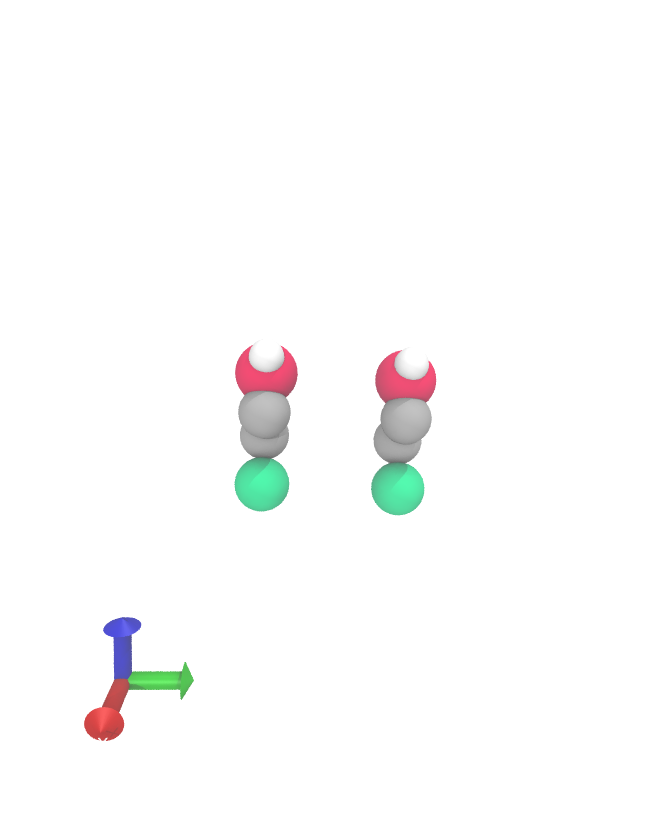
\includegraphics[trim=0 0 0 300,clip,width=0.5\textwidth]{two_meoh}
\end{figure}

Our MeOH molecules have the following coordinates:

\begin{align*}
  &S\ (0.138,0.0,-1.654)   &S'\ (0.138,5.0,-1.654)\\
  &C1\ (0.474,0.0,1.059)   &C1'\ (0.474,5.0,1.059)\\
  &C2\ (-0.621,0.0,-0.007) &C2'\ (-0.621,5.0,-0.007)\\
  &O\ (-0.125,0.0,2.357)   &O'\ (-0.125,5.0,2.357)\\
  &H\ (0.598,0.0,2.999)    &H'\ (0.598,5.0,2.999)\\
\end{align*}

\begin{knitrout}
\definecolor{shadecolor}{rgb}{0.969, 0.969, 0.969}\color{fgcolor}\begin{kframe}
\begin{alltt}
  \hlstd{S}\hlkwb{=}\hlkwd{c}\hlstd{(}\hlnum{2}\hlstd{,}\hlnum{0.0}\hlstd{,}\hlnum{0.138}\hlstd{,}\hlnum{0.0}\hlstd{,}\hlopt{-}\hlnum{1.654}\hlstd{)}
  \hlstd{C1}\hlkwb{=}\hlkwd{c}\hlstd{(}\hlnum{1}\hlstd{,}\hlnum{0.0}\hlstd{,}\hlnum{0.474}\hlstd{,}\hlnum{0.0}\hlstd{,}\hlnum{1.059}\hlstd{)}
  \hlstd{C2}\hlkwb{=}\hlkwd{c}\hlstd{(}\hlnum{1}\hlstd{,}\hlnum{0.265}\hlstd{,}\hlopt{-}\hlnum{0.621}\hlstd{,}\hlnum{0.0}\hlstd{,}\hlopt{-}\hlnum{0.007}\hlstd{)}
  \hlstd{O}\hlkwb{=}\hlkwd{c}\hlstd{(}\hlnum{3}\hlstd{,}\hlopt{-}\hlnum{0.700}\hlstd{,}\hlopt{-}\hlnum{0.125}\hlstd{,}\hlnum{0.0}\hlstd{,}\hlnum{2.357}\hlstd{)}
  \hlstd{H}\hlkwb{=}\hlkwd{c}\hlstd{(}\hlnum{4}\hlstd{,}\hlnum{0.435}\hlstd{,}\hlnum{0.598}\hlstd{,}\hlnum{0.0}\hlstd{,}\hlnum{2.999}\hlstd{)}
  \hlstd{S_2}\hlkwb{=}\hlkwd{c}\hlstd{(}\hlnum{2}\hlstd{,}\hlnum{0.0}\hlstd{,}\hlnum{0.138}\hlstd{,}\hlnum{5.0}\hlstd{,}\hlopt{-}\hlnum{1.654}\hlstd{)}
  \hlstd{C1_2}\hlkwb{=}\hlkwd{c}\hlstd{(}\hlnum{1}\hlstd{,}\hlnum{0.0}\hlstd{,}\hlnum{0.474}\hlstd{,}\hlnum{5.0}\hlstd{,}\hlnum{1.059}\hlstd{)}
  \hlstd{C2_2}\hlkwb{=}\hlkwd{c}\hlstd{(}\hlnum{1}\hlstd{,}\hlnum{0.265}\hlstd{,}\hlopt{-}\hlnum{0.621}\hlstd{,}\hlnum{5.0}\hlstd{,}\hlopt{-}\hlnum{0.007}\hlstd{)}
  \hlstd{O_2}\hlkwb{=}\hlkwd{c}\hlstd{(}\hlnum{3}\hlstd{,}\hlopt{-}\hlnum{0.700}\hlstd{,}\hlopt{-}\hlnum{0.125}\hlstd{,}\hlnum{5.0}\hlstd{,}\hlnum{2.357}\hlstd{)}
  \hlstd{H_2}\hlkwb{=}\hlkwd{c}\hlstd{(}\hlnum{4}\hlstd{,}\hlnum{0.435}\hlstd{,}\hlnum{0.598}\hlstd{,}\hlnum{5.0}\hlstd{,}\hlnum{2.999}\hlstd{)}
\end{alltt}
\end{kframe}
\end{knitrout}


Based on the number of atoms the total number of pairwise interactions are:

\[ \binom{N_{atoms}}{2}=\binom{10}{2} = 45 \]

Subtracting off the excluded intramolecular forces we have:

\[  \binom{N_{atoms}}{2}-2\cdot\binom{N_{atoms}/2}{2}+2=\binom{10}{2}-2\cdot\binom{5}{2}+2=27\]
The LJ Parameters are:

% latex table generated in R 3.3.3 by xtable 1.8-2 package
% Tue May 23 16:33:57 2017
\begin{table}[ht]
\centering
\begin{tabular}{|l||c||c|}
  \hline
Elements & Epsilons (kcal/mol) & Sigmas (A) \\ 
  \hline
C & 0.118 & 3.905 \\ 
  S & 0.397 & 4.250 \\ 
  O & 0.200 & 2.850 \\ 
  H & 0.000 & 1.780 \\ 
   \hline
\end{tabular}
\end{table}


Calculating the energies of all possible combinations we get:

\begin{knitrout}
\definecolor{shadecolor}{rgb}{0.969, 0.969, 0.969}\color{fgcolor}\begin{kframe}
\begin{alltt}
  \hlstd{distance}\hlkwb{=}\hlkwa{function}\hlstd{(}\hlkwc{atom1}\hlstd{,}\hlkwc{atom2}\hlstd{)\{}
    \hlkwd{return}\hlstd{(}\hlkwd{norm}\hlstd{(atom1[}\hlnum{3}\hlopt{:}\hlnum{5}\hlstd{]}\hlopt{-}\hlstd{atom2[}\hlnum{3}\hlopt{:}\hlnum{5}\hlstd{],}\hlkwc{type}\hlstd{=}\hlstr{"2"}\hlstd{))}
  \hlstd{\}}
  \hlstd{energy}\hlkwb{=}\hlkwa{function}\hlstd{(}\hlkwc{atom1}\hlstd{,}\hlkwc{atom2}\hlstd{)\{}
    \hlstd{r}\hlkwb{=}\hlkwd{distance}\hlstd{(atom1,atom2)}
    \hlstd{sigma} \hlkwb{=} \hlstd{(sigmas[atom1[}\hlnum{1}\hlstd{]]}\hlopt{+}\hlstd{sigmas[atom2[}\hlnum{1}\hlstd{]])}\hlopt{/}\hlnum{2}
    \hlstd{epsilon} \hlkwb{=} \hlkwd{sqrt}\hlstd{(epsilons[atom1[}\hlnum{1}\hlstd{]]}\hlopt{*}\hlstd{epsilons[atom2[}\hlnum{1}\hlstd{]])}
    \hlkwd{return}\hlstd{(}\hlnum{4}\hlopt{*}\hlstd{epsilon}\hlopt{*}\hlstd{((sigma}\hlopt{/}\hlstd{r)}\hlopt{^}\hlnum{12}\hlopt{-}\hlstd{(sigma}\hlopt{/}\hlstd{r)}\hlopt{^}\hlnum{6}\hlstd{))}
  \hlstd{\}}
  \hlstd{atoms} \hlkwb{=} \hlkwd{list}\hlstd{(S,C1,C2,O,H,S_2,C1_2,C2_2,O_2,H_2)}
  \hlstd{atom_combos} \hlkwb{=} \hlkwd{combn}\hlstd{(atoms,}\hlnum{2}\hlstd{)}
  \hlstd{distances}\hlkwb{=}\hlkwd{mapply}\hlstd{(distance,atom_combos[}\hlnum{1}\hlstd{,],atom_combos[}\hlnum{2}\hlstd{,])}
  \hlkwd{print}\hlstd{(distances)}
\end{alltt}
\begin{verbatim}
##  [1] 2.7337273 1.8134746 4.0196132 4.6756827 5.0000000 5.6985318 5.3187113
##  [8] 6.4153948 6.8455832 1.5281953 1.4295471 1.9439588 5.6985318 5.0000000
## [15] 5.2283249 5.2003466 5.3646040 2.4154735 3.2437628 5.3187113 5.2283249
## [22] 5.0000000 5.5528832 5.9600333 0.9668987 6.4153948 5.2003466 5.5528832
## [29] 5.0000000 5.0926312 6.8455832 5.3646040 5.9600333 5.0926312 5.0000000
## [36] 2.7337273 1.8134746 4.0196132 4.6756827 1.5281953 1.4295471 1.9439588
## [43] 2.4154735 3.2437628 0.9668987
\end{verbatim}
\begin{alltt}
  \hlstd{vdw_energies} \hlkwb{=} \hlkwd{mapply}\hlstd{(energy,atom_combos[,distances}\hlopt{>=}\hlnum{5}\hlstd{][}\hlnum{1}\hlstd{,],atom_combos[,distances}\hlopt{>=}\hlnum{5}\hlstd{][}\hlnum{2}\hlstd{,])}
  \hlkwd{print}\hlstd{(vdw_energies)}
\end{alltt}
\begin{verbatim}
##  [1] -0.37343756 -0.10065368 -0.14015464 -0.03144736  0.00000000
##  [6] -0.10065368 -0.08280619 -0.06771469 -0.04265897  0.00000000
## [11] -0.14015464 -0.06771469 -0.08280619 -0.02953994  0.00000000
## [16] -0.03144736 -0.04265897 -0.02953994 -0.02649616  0.00000000
## [21]  0.00000000  0.00000000  0.00000000  0.00000000  0.00000000
\end{verbatim}
\begin{alltt}
  \hlkwd{sprintf}\hlstd{(}\hlstr{"Total intermolecular Van der Waals Energy is: %4.4f kcal/mol"}\hlstd{,}\hlkwd{sum}\hlstd{(vdw_energies))}
\end{alltt}
\begin{verbatim}
## [1] "Total intermolecular Van der Waals Energy is: -1.3899 kcal/mol"
\end{verbatim}
\end{kframe}
\end{knitrout}

Therefore the total energy is given as the total intermolecular energy plus the intramolecular energy of the two MeOHs:

\begin{align*}
  \text{Total Van der Waals Energy}&=\text{Intermolecular Energy}+\text{Intramolecular Energy}\\
    &=-1.3898847+-0.2812=-1.6710847\ \text{kcal/mol}
\end{align*}

Now we use the following code to calculate the total coulombic energy:

\begin{knitrout}
\definecolor{shadecolor}{rgb}{0.969, 0.969, 0.969}\color{fgcolor}\begin{kframe}
\begin{alltt}
  \hlstd{coul_energy}\hlkwb{=}\hlkwa{function}\hlstd{(}\hlkwc{atom1}\hlstd{,}\hlkwc{atom2}\hlstd{)\{}
    \hlstd{r}\hlkwb{=}\hlkwd{distance}\hlstd{(atom1,atom2)}
    \hlstd{k}\hlkwb{=}\hlnum{0.2}
    \hlkwd{return}\hlstd{(}\hlnum{332.0636}\hlopt{*}\hlstd{((atom1[}\hlnum{2}\hlstd{]}\hlopt{*}\hlstd{atom2[}\hlnum{2}\hlstd{])}\hlopt{/}\hlstd{r)}\hlopt{*}\hlkwd{exp}\hlstd{(}\hlopt{-}\hlstd{k}\hlopt{*}\hlstd{r))}
  \hlstd{\}}
  \hlstd{charged_atoms} \hlkwb{=} \hlkwd{list}\hlstd{(C2,O,H,C2_2,O_2,H_2)}
  \hlstd{charge_combos} \hlkwb{=} \hlkwd{combn}\hlstd{(charged_atoms,}\hlnum{2}\hlstd{)}
  \hlstd{distances}\hlkwb{=}\hlkwd{mapply}\hlstd{(distance,charge_combos[}\hlnum{1}\hlstd{,],charge_combos[}\hlnum{2}\hlstd{,])}
  \hlkwd{print}\hlstd{(distances)}
\end{alltt}
\begin{verbatim}
##  [1] 2.4154735 3.2437628 5.0000000 5.5528832 5.9600333 0.9668987 5.5528832
##  [8] 5.0000000 5.0926312 5.9600333 5.0926312 5.0000000 2.4154735 3.2437628
## [15] 0.9668987
\end{verbatim}
\begin{alltt}
  \hlstd{coul_energies} \hlkwb{=} \hlkwd{mapply}\hlstd{(coul_energy,charge_combos[,distances}\hlopt{>=}\hlnum{5}\hlstd{][}\hlnum{1}\hlstd{,],charge_combos[,distances}\hlopt{>=}\hlnum{5}\hlstd{][}\hlnum{2}\hlstd{,])}
  \hlkwd{print}\hlstd{(}\hlkwd{sum}\hlstd{(coul_energies))}
\end{alltt}
\begin{verbatim}
## [1] 0.5628225
\end{verbatim}
\end{kframe}
\end{knitrout}

The coulombic energy calculated here is:

\begin{align*}
  \Aboxed{\text{Total Coulombic Energy}=0.5628225\ \text{kcal/mol}}
\end{align*}

Then total energy is:

$$-1.1082622\ \text{kcal/mol}$$



\section{Rotating CCOH Dihedral $\pi$ Radians}

The axis of rotation for the $CCOH$ dihedral is:

\begin{knitrout}
\definecolor{shadecolor}{rgb}{0.969, 0.969, 0.969}\color{fgcolor}\begin{kframe}
\begin{alltt}
  \hlkwd{library}\hlstd{(scatterplot3d)}
  \hlstd{axis} \hlkwb{=} \hlstd{O[}\hlnum{3}\hlopt{:}\hlnum{5}\hlstd{]}\hlopt{-}\hlstd{C2[}\hlnum{3}\hlopt{:}\hlnum{5}\hlstd{]}
  \hlkwd{message}\hlstd{(}\hlkwd{sprintf}\hlstd{(}\hlstr{"The axis of rotation is: %s"}\hlstd{,}\hlkwd{paste}\hlstd{(axis,}\hlkwc{collapse}\hlstd{=}\hlstr{", "}\hlstd{)))}
\end{alltt}


{\ttfamily\noindent\itshape\color{messagecolor}{\#\# The axis of rotation is: 0.496, 0, 2.364}}\begin{alltt}
  \hlstd{normaxis} \hlkwb{=} \hlstd{axis}\hlopt{/}\hlkwd{sqrt}\hlstd{(}\hlkwd{sum}\hlstd{(axis}\hlopt{^}\hlnum{2}\hlstd{))}
  \hlkwd{message}\hlstd{(}\hlkwd{sprintf}\hlstd{(}\hlstr{"The normed axis of rotation is: %s"}\hlstd{,}\hlkwd{paste}\hlstd{(normaxis,}\hlkwc{collapse} \hlstd{=} \hlstr{", "}\hlstd{)))}
\end{alltt}


{\ttfamily\noindent\itshape\color{messagecolor}{\#\# The normed axis of rotation is: 0.205342766021818, 0, 0.978690118700761}}\begin{alltt}
  \hlcom{#Plot the molecule using scatterplot3d}
  \hlstd{x} \hlkwb{=} \hlkwd{c}\hlstd{(S[}\hlnum{3}\hlstd{],C1[}\hlnum{3}\hlstd{],C2[}\hlnum{3}\hlstd{],O[}\hlnum{3}\hlstd{],H[}\hlnum{3}\hlstd{])}
  \hlstd{y} \hlkwb{=} \hlkwd{c}\hlstd{(S[}\hlnum{4}\hlstd{],C1[}\hlnum{4}\hlstd{],C2[}\hlnum{4}\hlstd{],O[}\hlnum{4}\hlstd{],H[}\hlnum{4}\hlstd{])}
  \hlstd{z} \hlkwb{=} \hlkwd{c}\hlstd{(S[}\hlnum{5}\hlstd{],C1[}\hlnum{5}\hlstd{],C2[}\hlnum{5}\hlstd{],O[}\hlnum{5}\hlstd{],H[}\hlnum{5}\hlstd{])}
  \hlcom{#data_frame = data.frame(x,y,z)}
  \hlkwd{scatterplot3d}\hlstd{(x,y,z,}\hlkwc{type} \hlstd{=} \hlstr{"l"}\hlstd{)}
\end{alltt}
\end{kframe}
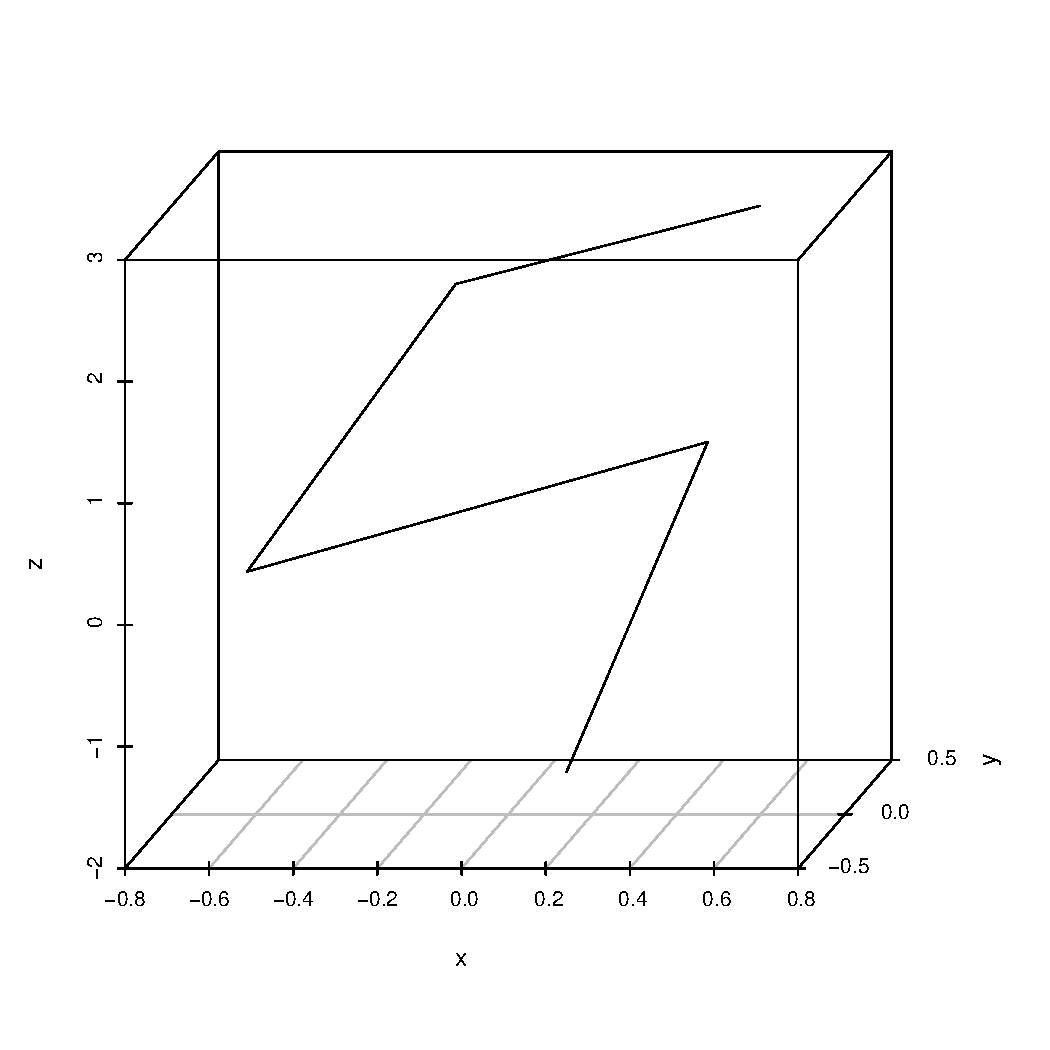
\includegraphics[width=\maxwidth]{figure/define-axis-1} 

\end{knitrout}

The quaternion that defines a $\pi$ radian rotation about this axis is:

$$\vec{q}=\cos(\frac{\theta}{2})+\sin(\frac{\theta}{2})\cdot\frac{1}{\| a \|}\vec{a}=\cos(\frac{\pi}{2})+\sin(\frac{\pi}{2})\cdot\frac{1}{\| a \|}\vec{a}$$

This turns out to be:

\begin{knitrout}
\definecolor{shadecolor}{rgb}{0.969, 0.969, 0.969}\color{fgcolor}\begin{kframe}
\begin{alltt}
\hlkwd{library}\hlstd{(onion)}
\hlstd{theta} \hlkwb{=} \hlstd{pi}
\hlstd{q} \hlkwb{=} \hlkwd{cos}\hlstd{(theta}\hlopt{/}\hlnum{2}\hlstd{)} \hlopt{+} \hlkwd{sin}\hlstd{(theta}\hlopt{/}\hlnum{2}\hlstd{)} \hlopt{*} \hlstd{normaxis[}\hlnum{1}\hlstd{]} \hlopt{*} \hlstd{Hi} \hlopt{+} \hlkwd{sin}\hlstd{(theta}\hlopt{/}\hlnum{2}\hlstd{)} \hlopt{*} \hlstd{normaxis[}\hlnum{2}\hlstd{]} \hlopt{*}
    \hlstd{Hj} \hlopt{+} \hlkwd{sin}\hlstd{(theta}\hlopt{/}\hlnum{2}\hlstd{)} \hlopt{*} \hlstd{normaxis[}\hlnum{3}\hlstd{]} \hlopt{*} \hlstd{Hk}
\hlkwd{message}\hlstd{(}\hlkwd{sprintf}\hlstd{(}\hlstr{"The quaternion of rotation is %s"}\hlstd{,} \hlkwd{paste}\hlstd{(q,} \hlkwc{collapse} \hlstd{=} \hlstr{", "}\hlstd{)))}
\end{alltt}


{\ttfamily\noindent\itshape\color{messagecolor}{\#\# The quaternion of rotation is 6.12303176911189e-17, 0.205342766021818, 0, 0.978690118700761}}\end{kframe}
\end{knitrout}

Finally we get the vectors we wish to rotate:

\begin{knitrout}
\definecolor{shadecolor}{rgb}{0.969, 0.969, 0.969}\color{fgcolor}\begin{kframe}
\begin{alltt}
\hlstd{v1} \hlkwb{=} \hlstd{H[}\hlnum{3}\hlopt{:}\hlnum{5}\hlstd{]} \hlopt{-} \hlstd{O[}\hlnum{3}\hlopt{:}\hlnum{5}\hlstd{]}
\hlkwd{message}\hlstd{(}\hlkwd{sprintf}\hlstd{(}\hlstr{"Vector 1 is %s"}\hlstd{,} \hlkwd{paste}\hlstd{(v1,} \hlkwc{collapse} \hlstd{=} \hlstr{", "}\hlstd{)))}
\end{alltt}


{\ttfamily\noindent\itshape\color{messagecolor}{\#\# Vector 1 is 0.723, 0, 0.642}}\end{kframe}
\end{knitrout}

Applying the rotation quaternions we get:

\begin{knitrout}
\definecolor{shadecolor}{rgb}{0.969, 0.969, 0.969}\color{fgcolor}\begin{kframe}
\begin{alltt}
\hlstd{v1_q} \hlkwb{=} \hlnum{0} \hlopt{+} \hlstd{v1[}\hlnum{1}\hlstd{]} \hlopt{*} \hlstd{Hi} \hlopt{+} \hlstd{v1[}\hlnum{2}\hlstd{]} \hlopt{*} \hlstd{Hj} \hlopt{+} \hlstd{v1[}\hlnum{3}\hlstd{]} \hlopt{*} \hlstd{Hk}
\hlstd{v1_rot_q} \hlkwb{=} \hlstd{(q} \hlopt{*} \hlstd{v1_q)} \hlopt{*} \hlkwd{Conj}\hlstd{(q)}
\hlstd{v1_rot} \hlkwb{=} \hlkwd{c}\hlstd{(}\hlkwd{i}\hlstd{(v1_rot_q),} \hlkwd{j}\hlstd{(v1_rot_q),} \hlkwd{k}\hlstd{(v1_rot_q))}
\hlkwd{message}\hlstd{(}\hlkwd{sprintf}\hlstd{(}\hlstr{"v1 rotated pi radians is now %s"}\hlstd{,} \hlkwd{paste}\hlstd{(v1_rot,} \hlkwc{collapse} \hlstd{=} \hlstr{", "}\hlstd{)))}
\end{alltt}


{\ttfamily\noindent\itshape\color{messagecolor}{\#\# v1 rotated pi radians is now -0.403986921956798, 7.05082905677622e-17, 0.878457492931714}}\end{kframe}
\end{knitrout}

This translates to final coordinates of O and H of:

\begin{knitrout}
\definecolor{shadecolor}{rgb}{0.969, 0.969, 0.969}\color{fgcolor}\begin{kframe}
\begin{alltt}
\hlstd{Hnew} \hlkwb{=} \hlkwd{c}\hlstd{(}\hlnum{4}\hlstd{,} \hlnum{0.435}\hlstd{, v1_rot} \hlopt{+} \hlstd{O[}\hlnum{3}\hlopt{:}\hlnum{5}\hlstd{])}
\hlkwd{message}\hlstd{(}\hlkwd{sprintf}\hlstd{(}\hlstr{"Hnew is %s"}\hlstd{,} \hlkwd{paste}\hlstd{(Hnew,} \hlkwc{collapse} \hlstd{=} \hlstr{","}\hlstd{)))}
\end{alltt}


{\ttfamily\noindent\itshape\color{messagecolor}{\#\# Hnew is 4,0.435,-0.528986921956798,7.05082905677622e-17,3.23545749293171}}\begin{alltt}
\hlcom{# Plot the new dihedral}
\hlstd{xnew} \hlkwb{=} \hlkwd{c}\hlstd{(S[}\hlnum{3}\hlstd{], C1[}\hlnum{3}\hlstd{], C2[}\hlnum{3}\hlstd{], O[}\hlnum{3}\hlstd{], Hnew[}\hlnum{3}\hlstd{])}
\hlstd{ynew} \hlkwb{=} \hlkwd{c}\hlstd{(S[}\hlnum{4}\hlstd{], C1[}\hlnum{4}\hlstd{], C2[}\hlnum{4}\hlstd{], O[}\hlnum{4}\hlstd{], Hnew[}\hlnum{4}\hlstd{])}
\hlstd{znew} \hlkwb{=} \hlkwd{c}\hlstd{(S[}\hlnum{5}\hlstd{], C1[}\hlnum{5}\hlstd{], C2[}\hlnum{5}\hlstd{], O[}\hlnum{5}\hlstd{], Hnew[}\hlnum{5}\hlstd{])}

\hlstd{xtotal} \hlkwb{=} \hlkwd{c}\hlstd{(x, xnew)}
\hlstd{ytotal} \hlkwb{=} \hlkwd{c}\hlstd{(y, ynew)}
\hlstd{ztotal} \hlkwb{=} \hlkwd{c}\hlstd{(z, znew)}
\hlstd{category} \hlkwb{=} \hlkwd{c}\hlstd{(}\hlkwd{rep}\hlstd{(}\hlstr{"blue"}\hlstd{,} \hlnum{5}\hlstd{),} \hlkwd{rep}\hlstd{(}\hlstr{"red"}\hlstd{,} \hlnum{5}\hlstd{))}
\hlstd{data_frame} \hlkwb{=} \hlkwd{data.frame}\hlstd{(xtotal, ytotal, ztotal)}
\hlstd{data_frame}\hlopt{$}\hlstd{fac} \hlkwb{=} \hlkwd{factor}\hlstd{(}\hlkwd{rep}\hlstd{(LETTERS[}\hlnum{1}\hlopt{:}\hlnum{2}\hlstd{],} \hlkwc{each} \hlstd{=} \hlnum{5}\hlstd{))}
\hlkwd{print}\hlstd{(}\hlkwd{c}\hlstd{(}\hlkwd{as.numeric}\hlstd{(data_frame}\hlopt{$}\hlstd{xtotal)))}
\end{alltt}
\begin{verbatim}
##  [1]  0.1380000  0.4740000 -0.6210000 -0.1250000  0.5980000  0.1380000
##  [7]  0.4740000 -0.6210000 -0.1250000 -0.5289869
\end{verbatim}
\begin{alltt}
\hlkwd{scatterplot3d}\hlstd{(}\hlkwc{x} \hlstd{= data_frame}\hlopt{$}\hlstd{xtotal,} \hlkwc{y} \hlstd{= data_frame}\hlopt{$}\hlstd{ytotal,} \hlkwc{z} \hlstd{= data_frame}\hlopt{$}\hlstd{ztotal)}
\end{alltt}


{\ttfamily\noindent\bfseries\color{errorcolor}{\#\# Error in plot.window(c(x1, x2), c(z.min, z.max + yz.f * y.max)): need finite 'xlim' values}}\end{kframe}

\includegraphics[width=\maxwidth]{figure/new-coords-1} 
\begin{kframe}\begin{alltt}
\hlcom{# ,type = 'l',color=as.numeric(data_frame$fac)}
\end{alltt}
\end{kframe}
\end{knitrout}

The calculated dihedral angle from these new coordinates is:

\begin{knitrout}
\definecolor{shadecolor}{rgb}{0.969, 0.969, 0.969}\color{fgcolor}\begin{kframe}
\begin{alltt}
\hlkwd{library}\hlstd{(pracma)}
\end{alltt}


{\ttfamily\noindent\itshape\color{messagecolor}{\#\# \\\#\# Attaching package: 'pracma'}}

{\ttfamily\noindent\itshape\color{messagecolor}{\#\# The following object is masked from 'package:onion':\\\#\# \\\#\#\ \ \ \  Norm}}\begin{alltt}
\hlstd{b1} \hlkwb{=} \hlstd{C2[}\hlnum{3}\hlopt{:}\hlnum{5}\hlstd{]} \hlopt{-} \hlstd{C1[}\hlnum{3}\hlopt{:}\hlnum{5}\hlstd{]}
\hlstd{b2} \hlkwb{=} \hlstd{O[}\hlnum{3}\hlopt{:}\hlnum{5}\hlstd{]} \hlopt{-} \hlstd{C2[}\hlnum{3}\hlopt{:}\hlnum{5}\hlstd{]}
\hlstd{b3} \hlkwb{=} \hlstd{Hnew[}\hlnum{3}\hlopt{:}\hlnum{5}\hlstd{]} \hlopt{-} \hlstd{O[}\hlnum{3}\hlopt{:}\hlnum{5}\hlstd{]}
\hlstd{b2norm} \hlkwb{=} \hlstd{b2}\hlopt{/}\hlkwd{sqrt}\hlstd{(}\hlkwd{sum}\hlstd{(b2}\hlopt{^}\hlnum{2}\hlstd{))}
\hlstd{n1} \hlkwb{=} \hlkwd{cross}\hlstd{(b1, b2)}\hlopt{/}\hlkwd{sqrt}\hlstd{(}\hlkwd{sum}\hlstd{(}\hlkwd{cross}\hlstd{(b1, b2)}\hlopt{^}\hlnum{2}\hlstd{))}
\hlstd{n2} \hlkwb{=} \hlkwd{cross}\hlstd{(b3, b2)}\hlopt{/}\hlkwd{sqrt}\hlstd{(}\hlkwd{sum}\hlstd{(}\hlkwd{cross}\hlstd{(b2, b3)}\hlopt{^}\hlnum{2}\hlstd{))}
\hlstd{m1} \hlkwb{=} \hlkwd{cross}\hlstd{(n1, n2)}
\hlstd{angle} \hlkwb{=} \hlkwd{atan2}\hlstd{((m1} \hlopt \hlstd{b2norm), (n1} \hlopt \hlstd{n2))}
\hlkwd{message}\hlstd{(}\hlkwd{sprintf}\hlstd{(}\hlstr{"The calculated dihedral angle of the resulting rotation is: %4.2f degrees"}\hlstd{,}
    \hlstd{angle} \hlopt{*} \hlnum{180}\hlopt{/}\hlstd{pi))}
\end{alltt}


{\ttfamily\noindent\itshape\color{messagecolor}{\#\# The calculated dihedral angle of the resulting rotation is: -0.00 degrees}}\end{kframe}
\end{knitrout}

The new energies are:

\begin{knitrout}
\definecolor{shadecolor}{rgb}{0.969, 0.969, 0.969}\color{fgcolor}\begin{kframe}
\begin{alltt}
  \hlstd{atoms} \hlkwb{=} \hlkwd{list}\hlstd{(S,C1,C2,O,Hnew,S_2,C1_2,C2_2,O_2,H_2)}
  \hlstd{atom_combos} \hlkwb{=} \hlkwd{combn}\hlstd{(atoms,}\hlnum{2}\hlstd{)}
  \hlstd{distances}\hlkwb{=}\hlkwd{mapply}\hlstd{(distance,atom_combos[}\hlnum{1}\hlstd{,],atom_combos[}\hlnum{2}\hlstd{,])}
  \hlkwd{print}\hlstd{(distances)}
\end{alltt}
\begin{verbatim}
##  [1] 2.7337273 1.8134746 4.0196132 4.9347407 5.0000000 5.6985318 5.3187113
##  [8] 6.4153948 6.8455832 1.5281953 1.4295471 2.3964453 5.6985318 5.0000000
## [15] 5.2283249 5.2003466 5.3646040 2.4154735 3.2437628 5.3187113 5.2283249
## [22] 5.0000000 5.5528832 5.9600333 0.9668987 6.4153948 5.2003466 5.5528832
## [29] 5.0000000 5.0926312 7.0250741 5.5446325 5.9600333 5.0926312 5.1308880
## [36] 2.7337273 1.8134746 4.0196132 4.6756827 1.5281953 1.4295471 1.9439588
## [43] 2.4154735 3.2437628 0.9668987
\end{verbatim}
\begin{alltt}
  \hlstd{vdw_energies} \hlkwb{=} \hlkwd{mapply}\hlstd{(energy,atom_combos[,distances}\hlopt{>=}\hlnum{5}\hlstd{][}\hlnum{1}\hlstd{,],atom_combos[,distances}\hlopt{>=}\hlnum{5}\hlstd{][}\hlnum{2}\hlstd{,])}
  \hlkwd{print}\hlstd{(vdw_energies)}
\end{alltt}
\begin{verbatim}
##  [1] -0.37343756 -0.10065368 -0.14015464 -0.03144736  0.00000000
##  [6] -0.10065368 -0.08280619 -0.06771469 -0.04265897  0.00000000
## [11] -0.14015464 -0.06771469 -0.08280619 -0.02953994  0.00000000
## [16] -0.03144736 -0.04265897 -0.02953994 -0.02649616  0.00000000
## [21]  0.00000000  0.00000000  0.00000000  0.00000000  0.00000000
\end{verbatim}
\begin{alltt}
  \hlkwd{print}\hlstd{(}\hlkwd{sum}\hlstd{(vdw_energies))}\hlopt{+}\hlstd{(}\hlnum{2}\hlopt{*-}\hlnum{0.1406}\hlstd{)}
\end{alltt}
\begin{verbatim}
## [1] -1.389885
## [1] -1.671085
\end{verbatim}
\begin{alltt}
  \hlstd{charged_atoms} \hlkwb{=} \hlkwd{list}\hlstd{(C2,O,Hnew,C2_2,O_2,H_2)}
  \hlstd{charge_combos} \hlkwb{=} \hlkwd{combn}\hlstd{(charged_atoms,}\hlnum{2}\hlstd{)}
  \hlstd{distances}\hlkwb{=}\hlkwd{mapply}\hlstd{(distance,charge_combos[}\hlnum{1}\hlstd{,],charge_combos[}\hlnum{2}\hlstd{,])}
  \hlkwd{print}\hlstd{(distances)}
\end{alltt}
\begin{verbatim}
##  [1] 2.4154735 3.2437628 5.0000000 5.5528832 5.9600333 0.9668987 5.5528832
##  [8] 5.0000000 5.0926312 5.9600333 5.0926312 5.1308880 2.4154735 3.2437628
## [15] 0.9668987
\end{verbatim}
\begin{alltt}
  \hlstd{coul_energies} \hlkwb{=} \hlkwd{mapply}\hlstd{(coul_energy,charge_combos[,distances}\hlopt{>=}\hlnum{4.4}\hlstd{][}\hlnum{1}\hlstd{,],charge_combos[,distances}\hlopt{>=}\hlnum{4.4}\hlstd{][}\hlnum{2}\hlstd{,])}
  \hlkwd{print}\hlstd{(coul_energies)}
\end{alltt}
\begin{verbatim}
## [1]  1.715728 -3.653670  1.949960 -3.653670 11.971618 -7.170113  1.949960
## [8] -7.170113  4.388782
\end{verbatim}
\begin{alltt}
  \hlkwd{print}\hlstd{(}\hlkwd{sum}\hlstd{(coul_energies))}
\end{alltt}
\begin{verbatim}
## [1] 0.3284828
\end{verbatim}
\begin{alltt}
  \hlkwd{sprintf}\hlstd{(}\hlstr{"Total energy is %4.8f kcal/mol"}\hlstd{,}\hlkwd{sum}\hlstd{(coul_energies)}\hlopt{+}\hlkwd{sum}\hlstd{(vdw_energies)}\hlopt{+}\hlstd{(}\hlnum{2}\hlopt{*-}\hlnum{0.1406}\hlstd{))}
\end{alltt}
\begin{verbatim}
## [1] "Total energy is -1.34260189 kcal/mol"
\end{verbatim}
\end{kframe}
\end{knitrout}

\section{Rotating CCOH Dihedral $\frac{\pi}{2}$ Radians}

The axis of rotation for the $CCOH$ dihedral is:

\begin{knitrout}
\definecolor{shadecolor}{rgb}{0.969, 0.969, 0.969}\color{fgcolor}\begin{kframe}
\begin{alltt}
  \hlkwd{library}\hlstd{(scatterplot3d)}
  \hlstd{axis} \hlkwb{=} \hlstd{O[}\hlnum{3}\hlopt{:}\hlnum{5}\hlstd{]}\hlopt{-}\hlstd{C2[}\hlnum{3}\hlopt{:}\hlnum{5}\hlstd{]}
  \hlkwd{message}\hlstd{(}\hlkwd{sprintf}\hlstd{(}\hlstr{"The axis of rotation is: %s"}\hlstd{,}\hlkwd{paste}\hlstd{(axis,}\hlkwc{collapse}\hlstd{=}\hlstr{", "}\hlstd{)))}
\end{alltt}


{\ttfamily\noindent\itshape\color{messagecolor}{\#\# The axis of rotation is: 0.496, 0, 2.364}}\begin{alltt}
  \hlstd{normaxis} \hlkwb{=} \hlstd{axis}\hlopt{/}\hlkwd{sqrt}\hlstd{(}\hlkwd{sum}\hlstd{(axis}\hlopt{^}\hlnum{2}\hlstd{))}
  \hlkwd{message}\hlstd{(}\hlkwd{sprintf}\hlstd{(}\hlstr{"The normed axis of rotation is: %s"}\hlstd{,}\hlkwd{paste}\hlstd{(normaxis,}\hlkwc{collapse} \hlstd{=} \hlstr{", "}\hlstd{)))}
\end{alltt}


{\ttfamily\noindent\itshape\color{messagecolor}{\#\# The normed axis of rotation is: 0.205342766021818, 0, 0.978690118700761}}\begin{alltt}
  \hlcom{#Plot the molecule using scatterplot3d}
  \hlstd{x} \hlkwb{=} \hlkwd{c}\hlstd{(S[}\hlnum{3}\hlstd{],C1[}\hlnum{3}\hlstd{],C2[}\hlnum{3}\hlstd{],O[}\hlnum{3}\hlstd{],H[}\hlnum{3}\hlstd{])}
  \hlstd{y} \hlkwb{=} \hlkwd{c}\hlstd{(S[}\hlnum{4}\hlstd{],C1[}\hlnum{4}\hlstd{],C2[}\hlnum{4}\hlstd{],O[}\hlnum{4}\hlstd{],H[}\hlnum{4}\hlstd{])}
  \hlstd{z} \hlkwb{=} \hlkwd{c}\hlstd{(S[}\hlnum{5}\hlstd{],C1[}\hlnum{5}\hlstd{],C2[}\hlnum{5}\hlstd{],O[}\hlnum{5}\hlstd{],H[}\hlnum{5}\hlstd{])}
  \hlcom{#data_frame = data.frame(x,y,z)}
  \hlkwd{scatterplot3d}\hlstd{(x,y,z,}\hlkwc{type} \hlstd{=} \hlstr{"l"}\hlstd{)}
\end{alltt}
\end{kframe}
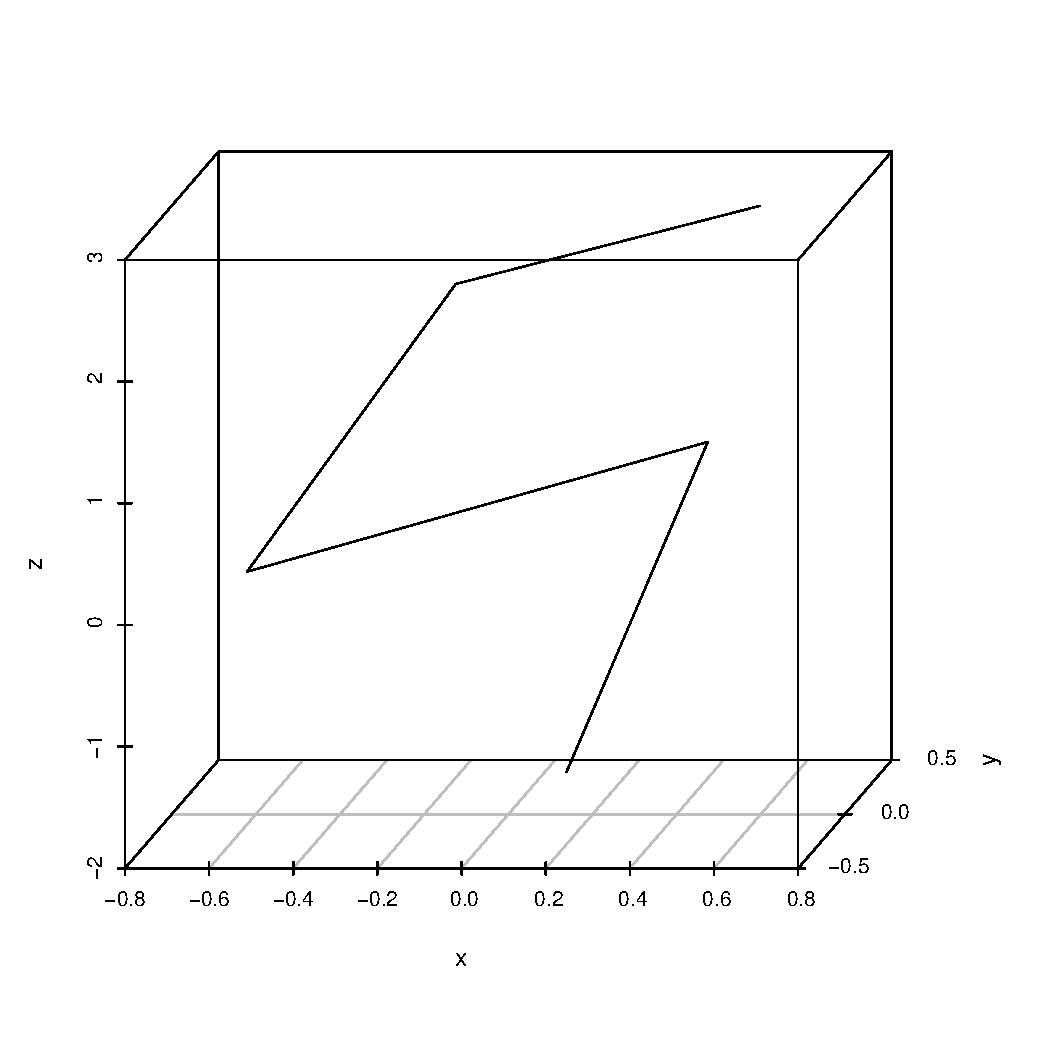
\includegraphics[width=\maxwidth]{figure/define-axis-pi-div-2-1} 

\end{knitrout}

The quaternion that defines a $\frac{\pi}{2}$ radian rotation about this axis is:

$$\vec{q}=\cos(\frac{\theta}{2})+\sin(\frac{\theta}{2})\cdot\frac{1}{\| a \|}\vec{a}=\cos(\frac{\pi}{4})+\sin(\frac{\pi}{4})\cdot\frac{1}{\| a \|}\vec{a}$$

This turns out to be:

\begin{knitrout}
\definecolor{shadecolor}{rgb}{0.969, 0.969, 0.969}\color{fgcolor}\begin{kframe}
\begin{alltt}
\hlkwd{library}\hlstd{(onion)}
\hlstd{theta} \hlkwb{=} \hlstd{pi}\hlopt{/}\hlnum{2}
\hlstd{q} \hlkwb{=} \hlkwd{cos}\hlstd{(theta}\hlopt{/}\hlnum{2}\hlstd{)} \hlopt{+} \hlkwd{sin}\hlstd{(theta}\hlopt{/}\hlnum{2}\hlstd{)} \hlopt{*} \hlstd{normaxis[}\hlnum{1}\hlstd{]} \hlopt{*} \hlstd{Hi} \hlopt{+} \hlkwd{sin}\hlstd{(theta}\hlopt{/}\hlnum{2}\hlstd{)} \hlopt{*} \hlstd{normaxis[}\hlnum{2}\hlstd{]} \hlopt{*}
    \hlstd{Hj} \hlopt{+} \hlkwd{sin}\hlstd{(theta}\hlopt{/}\hlnum{2}\hlstd{)} \hlopt{*} \hlstd{normaxis[}\hlnum{3}\hlstd{]} \hlopt{*} \hlstd{Hk}
\hlkwd{message}\hlstd{(}\hlkwd{sprintf}\hlstd{(}\hlstr{"The quaternion of rotation is %s"}\hlstd{,} \hlkwd{paste}\hlstd{(q,} \hlkwc{collapse} \hlstd{=} \hlstr{", "}\hlstd{)))}
\end{alltt}


{\ttfamily\noindent\itshape\color{messagecolor}{\#\# The quaternion of rotation is 0.707106781186548, 0.14519926232163, 0, 0.692038419613575}}\end{kframe}
\end{knitrout}

Finally we get the vectors we wish to rotate:

\begin{knitrout}
\definecolor{shadecolor}{rgb}{0.969, 0.969, 0.969}\color{fgcolor}\begin{kframe}
\begin{alltt}
\hlstd{v1} \hlkwb{=} \hlstd{H[}\hlnum{3}\hlopt{:}\hlnum{5}\hlstd{]} \hlopt{-} \hlstd{O[}\hlnum{3}\hlopt{:}\hlnum{5}\hlstd{]}
\hlkwd{message}\hlstd{(}\hlkwd{sprintf}\hlstd{(}\hlstr{"Vector 1 is %s"}\hlstd{,} \hlkwd{paste}\hlstd{(v1,} \hlkwc{collapse} \hlstd{=} \hlstr{", "}\hlstd{)))}
\end{alltt}


{\ttfamily\noindent\itshape\color{messagecolor}{\#\# Vector 1 is 0.723, 0, 0.642}}\end{kframe}
\end{knitrout}

Applying the rotation quaternions we get:

\begin{knitrout}
\definecolor{shadecolor}{rgb}{0.969, 0.969, 0.969}\color{fgcolor}\begin{kframe}
\begin{alltt}
\hlstd{v1_q} \hlkwb{=} \hlnum{0} \hlopt{+} \hlstd{v1[}\hlnum{1}\hlstd{]} \hlopt{*} \hlstd{Hi} \hlopt{+} \hlstd{v1[}\hlnum{2}\hlstd{]} \hlopt{*} \hlstd{Hj} \hlopt{+} \hlstd{v1[}\hlnum{3}\hlstd{]} \hlopt{*} \hlstd{Hk}
\hlstd{v1_rot_q} \hlkwb{=} \hlstd{(q} \hlopt{*} \hlstd{v1_q)} \hlopt{*} \hlkwd{Conj}\hlstd{(q)}
\hlstd{v1_rot} \hlkwb{=} \hlkwd{c}\hlstd{(}\hlkwd{i}\hlstd{(v1_rot_q),} \hlkwd{j}\hlstd{(v1_rot_q),} \hlkwd{k}\hlstd{(v1_rot_q))}
\hlkwd{message}\hlstd{(}\hlkwd{sprintf}\hlstd{(}\hlstr{"v1 rotated pi radians is now %s"}\hlstd{,} \hlkwd{paste}\hlstd{(v1_rot,} \hlkwc{collapse} \hlstd{=} \hlstr{", "}\hlstd{)))}
\end{alltt}


{\ttfamily\noindent\itshape\color{messagecolor}{\#\# v1 rotated pi radians is now 0.159506539021601, 0.575762900034643, 0.760228746465857}}\end{kframe}
\end{knitrout}

This translates to final coordinates of O and H of:

\begin{knitrout}
\definecolor{shadecolor}{rgb}{0.969, 0.969, 0.969}\color{fgcolor}\begin{kframe}
\begin{alltt}
\hlstd{Hnew} \hlkwb{=} \hlkwd{c}\hlstd{(}\hlnum{4}\hlstd{,} \hlnum{0.435}\hlstd{, v1_rot} \hlopt{+} \hlstd{O[}\hlnum{3}\hlopt{:}\hlnum{5}\hlstd{])}
\hlkwd{message}\hlstd{(}\hlkwd{sprintf}\hlstd{(}\hlstr{"Hnew is %s"}\hlstd{,} \hlkwd{paste}\hlstd{(Hnew,} \hlkwc{collapse} \hlstd{=} \hlstr{","}\hlstd{)))}
\end{alltt}


{\ttfamily\noindent\itshape\color{messagecolor}{\#\# Hnew is 4,0.435,0.0345065390216012,0.575762900034643,3.11722874646586}}\begin{alltt}
\hlcom{# Plot the new dihedral}
\hlstd{xnew} \hlkwb{=} \hlkwd{c}\hlstd{(S[}\hlnum{3}\hlstd{], C1[}\hlnum{3}\hlstd{], C2[}\hlnum{3}\hlstd{], O[}\hlnum{3}\hlstd{], Hnew[}\hlnum{3}\hlstd{])}
\hlstd{ynew} \hlkwb{=} \hlkwd{c}\hlstd{(S[}\hlnum{4}\hlstd{], C1[}\hlnum{4}\hlstd{], C2[}\hlnum{4}\hlstd{], O[}\hlnum{4}\hlstd{], Hnew[}\hlnum{4}\hlstd{])}
\hlstd{znew} \hlkwb{=} \hlkwd{c}\hlstd{(S[}\hlnum{5}\hlstd{], C1[}\hlnum{5}\hlstd{], C2[}\hlnum{5}\hlstd{], O[}\hlnum{5}\hlstd{], Hnew[}\hlnum{5}\hlstd{])}

\hlstd{xtotal} \hlkwb{=} \hlkwd{c}\hlstd{(x, xnew)}
\hlstd{ytotal} \hlkwb{=} \hlkwd{c}\hlstd{(y, ynew)}
\hlstd{ztotal} \hlkwb{=} \hlkwd{c}\hlstd{(z, znew)}
\hlstd{category} \hlkwb{=} \hlkwd{c}\hlstd{(}\hlkwd{rep}\hlstd{(}\hlstr{"blue"}\hlstd{,} \hlnum{5}\hlstd{),} \hlkwd{rep}\hlstd{(}\hlstr{"red"}\hlstd{,} \hlnum{5}\hlstd{))}
\hlstd{data_frame} \hlkwb{=} \hlkwd{data.frame}\hlstd{(xtotal, ytotal, ztotal)}
\hlstd{data_frame}\hlopt{$}\hlstd{fac} \hlkwb{=} \hlkwd{factor}\hlstd{(}\hlkwd{rep}\hlstd{(LETTERS[}\hlnum{1}\hlopt{:}\hlnum{2}\hlstd{],} \hlkwc{each} \hlstd{=} \hlnum{5}\hlstd{))}
\hlkwd{print}\hlstd{(}\hlkwd{c}\hlstd{(}\hlkwd{as.numeric}\hlstd{(data_frame}\hlopt{$}\hlstd{xtotal)))}
\end{alltt}
\begin{verbatim}
##  [1]  0.13800000  0.47400000 -0.62100000 -0.12500000  0.59800000
##  [6]  0.13800000  0.47400000 -0.62100000 -0.12500000  0.03450654
\end{verbatim}
\begin{alltt}
\hlkwd{scatterplot3d}\hlstd{(}\hlkwc{x} \hlstd{= data_frame}\hlopt{$}\hlstd{xtotal,} \hlkwc{y} \hlstd{= data_frame}\hlopt{$}\hlstd{ytotal,} \hlkwc{z} \hlstd{= data_frame}\hlopt{$}\hlstd{ztotal)}
\end{alltt}
\end{kframe}
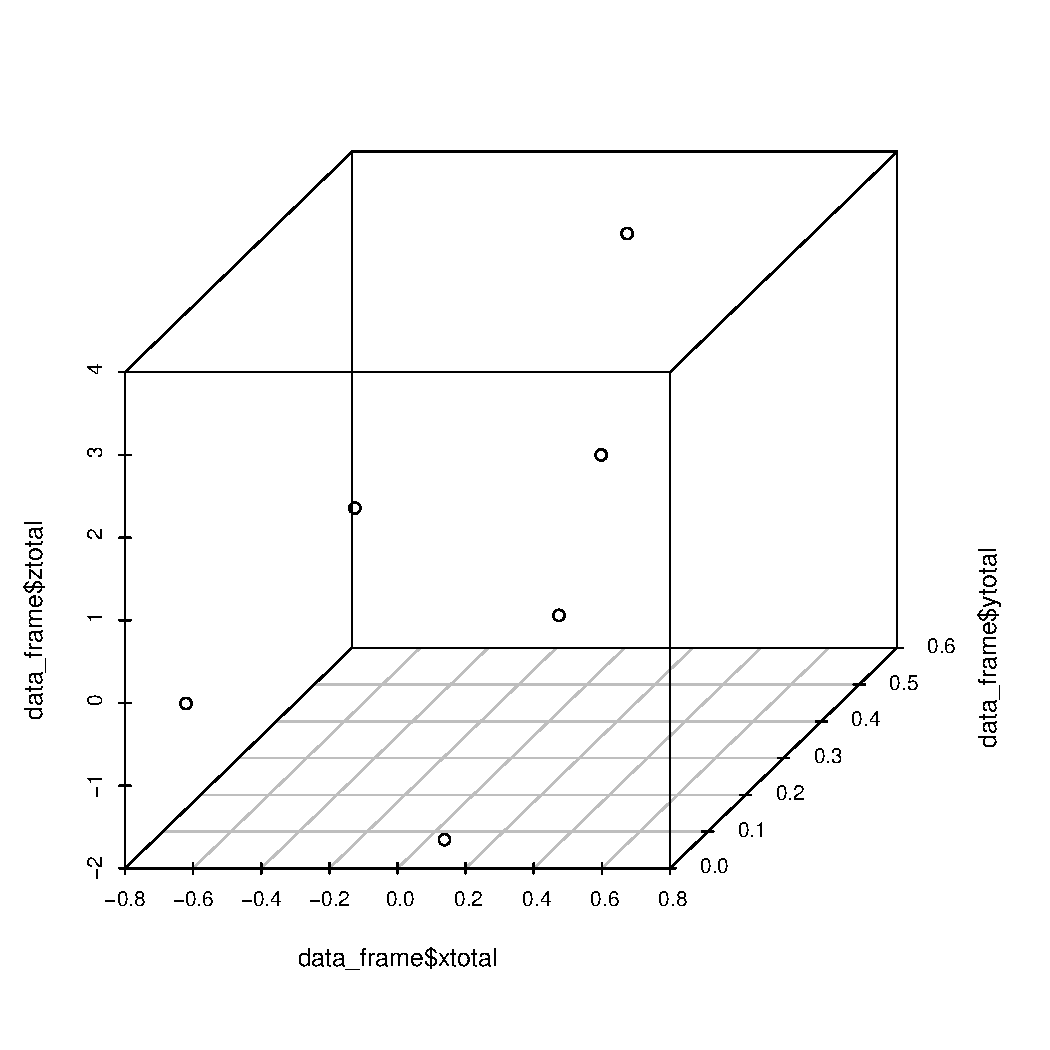
\includegraphics[width=\maxwidth]{figure/new-coords-pi-div-2-1} 
\begin{kframe}\begin{alltt}
\hlcom{# ,type = 'l',color=as.numeric(data_frame$fac)}
\end{alltt}
\end{kframe}
\end{knitrout}

The calculated dihedral angle from these new coordinates is:

\begin{knitrout}
\definecolor{shadecolor}{rgb}{0.969, 0.969, 0.969}\color{fgcolor}\begin{kframe}
\begin{alltt}
\hlkwd{library}\hlstd{(pracma)}
\hlstd{b1} \hlkwb{=} \hlstd{C2[}\hlnum{3}\hlopt{:}\hlnum{5}\hlstd{]} \hlopt{-} \hlstd{C1[}\hlnum{3}\hlopt{:}\hlnum{5}\hlstd{]}
\hlstd{b2} \hlkwb{=} \hlstd{O[}\hlnum{3}\hlopt{:}\hlnum{5}\hlstd{]} \hlopt{-} \hlstd{C2[}\hlnum{3}\hlopt{:}\hlnum{5}\hlstd{]}
\hlstd{b3} \hlkwb{=} \hlstd{Hnew[}\hlnum{3}\hlopt{:}\hlnum{5}\hlstd{]} \hlopt{-} \hlstd{O[}\hlnum{3}\hlopt{:}\hlnum{5}\hlstd{]}
\hlstd{b2norm} \hlkwb{=} \hlstd{b2}\hlopt{/}\hlkwd{sqrt}\hlstd{(}\hlkwd{sum}\hlstd{(b2}\hlopt{^}\hlnum{2}\hlstd{))}
\hlstd{n1} \hlkwb{=} \hlkwd{cross}\hlstd{(b1, b2)}\hlopt{/}\hlkwd{sqrt}\hlstd{(}\hlkwd{sum}\hlstd{(}\hlkwd{cross}\hlstd{(b1, b2)}\hlopt{^}\hlnum{2}\hlstd{))}
\hlstd{n2} \hlkwb{=} \hlkwd{cross}\hlstd{(b3, b2)}\hlopt{/}\hlkwd{sqrt}\hlstd{(}\hlkwd{sum}\hlstd{(}\hlkwd{cross}\hlstd{(b2, b3)}\hlopt{^}\hlnum{2}\hlstd{))}
\hlstd{m1} \hlkwb{=} \hlkwd{cross}\hlstd{(n1, n2)}
\hlstd{angle} \hlkwb{=} \hlkwd{atan2}\hlstd{((m1} \hlopt \hlstd{b2norm), (n1} \hlopt \hlstd{n2))}
\hlkwd{message}\hlstd{(}\hlkwd{sprintf}\hlstd{(}\hlstr{"The calculated dihedral angle of the resulting rotation is: %4.2f degrees"}\hlstd{,}
    \hlstd{angle} \hlopt{*} \hlnum{180}\hlopt{/}\hlstd{pi))}
\end{alltt}


{\ttfamily\noindent\itshape\color{messagecolor}{\#\# The calculated dihedral angle of the resulting rotation is: -90.00 degrees}}\end{kframe}
\end{knitrout}

The new energies are:

\begin{knitrout}
\definecolor{shadecolor}{rgb}{0.969, 0.969, 0.969}\color{fgcolor}\begin{kframe}
\begin{alltt}
  \hlstd{atoms} \hlkwb{=} \hlkwd{list}\hlstd{(S,C1,C2,O,Hnew,S_2,C1_2,C2_2,O_2,H_2)}
  \hlstd{atom_combos} \hlkwb{=} \hlkwd{combn}\hlstd{(atoms,}\hlnum{2}\hlstd{)}
  \hlstd{distances}\hlkwb{=}\hlkwd{mapply}\hlstd{(distance,atom_combos[}\hlnum{1}\hlstd{,],atom_combos[}\hlnum{2}\hlstd{,])}
  \hlkwd{print}\hlstd{(distances)}
\end{alltt}
\begin{verbatim}
##  [1] 2.7337273 1.8134746 4.0196132 4.8069572 5.0000000 5.6985318 5.3187113
##  [8] 6.4153948 6.8455832 1.5281953 1.4295471 2.1819631 5.6985318 5.0000000
## [15] 5.2283249 5.2003466 5.3646040 2.4154735 3.2437628 5.3187113 5.2283249
## [22] 5.0000000 5.5528832 5.9600333 0.9668987 6.4153948 5.2003466 5.5528832
## [29] 5.0000000 5.0926312 6.5076270 4.8993197 5.4556730 4.4919110 4.4615442
## [36] 2.7337273 1.8134746 4.0196132 4.6756827 1.5281953 1.4295471 1.9439588
## [43] 2.4154735 3.2437628 0.9668987
\end{verbatim}
\begin{alltt}
  \hlstd{vdw_energies} \hlkwb{=} \hlkwd{mapply}\hlstd{(energy,atom_combos[,distances}\hlopt{>=}\hlnum{5}\hlstd{][}\hlnum{1}\hlstd{,],atom_combos[,distances}\hlopt{>=}\hlnum{5}\hlstd{][}\hlnum{2}\hlstd{,])}
  \hlkwd{print}\hlstd{(vdw_energies)}
\end{alltt}
\begin{verbatim}
##  [1] -0.37343756 -0.10065368 -0.14015464 -0.03144736  0.00000000
##  [6] -0.10065368 -0.08280619 -0.06771469 -0.04265897  0.00000000
## [11] -0.14015464 -0.06771469 -0.08280619 -0.02953994  0.00000000
## [16] -0.03144736 -0.04265897 -0.02953994 -0.02649616  0.00000000
## [21]  0.00000000  0.00000000
\end{verbatim}
\begin{alltt}
  \hlkwd{print}\hlstd{(}\hlkwd{sum}\hlstd{(vdw_energies))}\hlopt{+}\hlstd{(}\hlnum{2}\hlopt{*-}\hlnum{0.1406}\hlstd{)}
\end{alltt}
\begin{verbatim}
## [1] -1.389885
## [1] -1.671085
\end{verbatim}
\begin{alltt}
  \hlstd{charged_atoms} \hlkwb{=} \hlkwd{list}\hlstd{(C2,O,Hnew,C2_2,O_2,H_2)}
  \hlstd{charge_combos} \hlkwb{=} \hlkwd{combn}\hlstd{(charged_atoms,}\hlnum{2}\hlstd{)}
  \hlstd{distances}\hlkwb{=}\hlkwd{mapply}\hlstd{(distance,charge_combos[}\hlnum{1}\hlstd{,],charge_combos[}\hlnum{2}\hlstd{,])}
  \hlkwd{print}\hlstd{(distances)}
\end{alltt}
\begin{verbatim}
##  [1] 2.4154735 3.2437628 5.0000000 5.5528832 5.9600333 0.9668987 5.5528832
##  [8] 5.0000000 5.0926312 5.4556730 4.4919110 4.4615442 2.4154735 3.2437628
## [15] 0.9668987
\end{verbatim}
\begin{alltt}
  \hlstd{coul_energies} \hlkwb{=} \hlkwd{mapply}\hlstd{(coul_energy,charge_combos[,distances}\hlopt{>=}\hlnum{4.4}\hlstd{][}\hlnum{1}\hlstd{,],charge_combos[,distances}\hlopt{>=}\hlnum{4.4}\hlstd{][}\hlnum{2}\hlstd{,])}
  \hlkwd{print}\hlstd{(coul_energies)}
\end{alltt}
\begin{verbatim}
## [1]  1.715728 -3.653670  1.949960 -3.653670 11.971618 -7.170113  2.356320
## [8] -9.166742  5.770186
\end{verbatim}
\begin{alltt}
  \hlkwd{print}\hlstd{(}\hlkwd{sum}\hlstd{(coul_energies))}
\end{alltt}
\begin{verbatim}
## [1] 0.1196177
\end{verbatim}
\begin{alltt}
  \hlkwd{sprintf}\hlstd{(}\hlstr{"Total energy is %4.8f kcal/mol"}\hlstd{,}\hlkwd{sum}\hlstd{(coul_energies)}\hlopt{+}\hlkwd{sum}\hlstd{(vdw_energies)}\hlopt{+}\hlstd{(}\hlnum{2}\hlopt{*-}\hlnum{0.1406}\hlstd{))}
\end{alltt}
\begin{verbatim}
## [1] "Total energy is -1.55146693 kcal/mol"
\end{verbatim}
\end{kframe}
\end{knitrout}

\end{document}


























